\documentclass[10pt]{article}
\usepackage[letterpaper,margin=1in]{geometry}
\usepackage{times}
\usepackage[T1]{fontenc}
\usepackage[utf8]{inputenc}
\usepackage{amsmath,amssymb,amsthm,mathtools,bm}
\usepackage{booktabs,multirow,graphicx,xcolor}
\usepackage[numbers,sort&compress]{natbib}
\usepackage{microtype}
\usepackage[colorlinks=true,linkcolor=blue!50!black,citecolor=blue!50!black,urlcolor=blue!50!black]{hyperref}
\usepackage[capitalise,noabbrev]{cleveref}
\usepackage{algorithm}
\usepackage{algpseudocode}
\usepackage{caption}
\captionsetup{font=small}
\newtheorem{proposition}{Proposition}
\newtheorem{remark}{Remark}
\newcommand{\R}{\mathbb{R}}
\newcommand{\Z}{\mathbb{Z}}
\newcommand{\cone}{\mathcal{K}}
\DeclareMathOperator*{\argmin}{arg\,min}
\newcommand{\OURgapA}{0.176}
\newcommand{\OURdiscA}{4.31}
\newcommand{\OURcontA}{7.51}
\newcommand{\PXgapA}{0.104}
\newcommand{\PXdiscA}{2.44}
\newcommand{\PXcontA}{4.28}
\newcommand{\OURtimeA}{3.3}
\newcommand{\PXtimeA}{3.5}
\newcommand{\REFtimeA}{78.3}
\newcommand{\SPDA}{24}
\newcommand{\OURgapB}{0.061}
\newcommand{\OURdiscB}{2.91}
\newcommand{\OURcontB}{3.46}
\newcommand{\PXgapB}{0.075}
\newcommand{\PXdiscB}{2.30}
\newcommand{\PXcontB}{2.87}
\newcommand{\OURtimeB}{31.9}
\newcommand{\PXtimeB}{31.2}
\newcommand{\REFtimeB}{346.6}
\newcommand{\SPDB}{11}
\newcommand{\OURgapV}{0.123}
\newcommand{\OURdiscV}{2.93}
\newcommand{\OURcontV}{3.03}
\newcommand{\PXgapV}{1.818}
\newcommand{\PXdiscV}{12.09}
\newcommand{\PXcontV}{10.27}
\newcommand{\OURtimeV}{0.011}
\newcommand{\PXtimeV}{0.039}
\newcommand{\REFtimeV}{0.99}
\newcommand{\SPDV}{92}
\newcommand{\VRATIO}{15}
\newcommand{\LABELHA}{4.0}
\newcommand{\TRAINA}{4{,}220}
\newcommand{\LABELHB}{13.2}
\newcommand{\TRAINB}{6{,}226}
\newcommand{\LABELSV}{147}
\newcommand{\TRAINV}{1{,}420}


\title{Self-Supervised Learning of Parametric Cutting Planes\\for Mixed-Integer Nonlinear Programs\\through Exact Differentiable Optimization Layers}
\author{Parth Brahmbhatt\\University of Wisconsin--Madison\\\texttt{prbrahmbhatt@wisc.edu}}
\date{}

\begin{document}
\maketitle

\begin{abstract}
Many online decision problems are parametric mixed-integer nonlinear programs (MINLPs) that must be re-solved every time their inputs change, yet are too expensive to solve exactly in real time.
A promising surrogate is a convex relaxation tightened by \emph{learned, parametric cutting planes}: a model maps the instance parameters to linear inequalities, and the cut relaxation is solved instead of the MINLP.
Dixit, Gupta and Zhang~\citep{dixit2025dfsm} learned such cuts for mixed-integer \emph{linear} programs by solving a large bilevel program whose lower levels are replaced by their KKT conditions, supervised by the optimal solutions of the original problem.
We instead place the cut relaxation \emph{inside} a neural network as an exact differentiable conic optimization layer and train the cut generator by stochastic gradient descent on the cost of the solution it ultimately deploys.
Training is \emph{self-supervised}: no optimal solutions are computed for training or model selection.
Making this work required (i) a two-layer differentiable deployment map (relaxation $\to$ soft rounding $\to$ continuous re-solve) whose gradient is exact rather than smoothed, (ii) a reverse-mode conic layer that remains accurate when the KKT system is singular, a regime in which \texttt{cvxpylayers} returns a 97\%-wrong gradient on our problems, and (iii) a depth-anchored cut parameterization that keeps every cut active, and therefore trainable, from initialization.
For nonconvex problems the same network also predicts the linearization point of the convexification.
We evaluate on AC unit commitment on the IEEE 118- and 300-bus systems (54 and 69 binaries, nonconvex AC physics) and on a convex hybrid-vehicle MINLP with 30 integer modes.
The learned surrogate deploys in \OURtimeA\,s, \OURtimeB\,s and \OURtimeV\,s per instance, \SPDA$\times$, \SPDB$\times$ and \SPDV$\times$ faster than the reference solvers, with mean cost deviations of \OURgapA\%, \OURgapB\% and \OURgapV\%.
Against a supervised neural-network proxy that is given the reference solutions and the same feasibility restoration, the learned cut is \VRATIO$\times$ more accurate in cost on the vehicle problem; on AC unit commitment the proxy is more accurate on case118, while on case300 the learned cut attains the lower cost deviation (\OURgapB\% vs.\ \PXgapB\%) and the proxy the lower decision errors. Our method uses none of the \LABELHA\,h (case118) and \LABELHB\,h (case300) of reference solves that the proxy is trained on.
\end{abstract}

\section{Introduction}
\label{sec:intro}

Unit commitment, energy management and hybrid-powertrain control are solved repeatedly, every few minutes or seconds, with only some parameters changing between solves: loads, prices, driver demand.
Each solve is a mixed-integer program, often with nonlinear physics, and a global solve can take minutes.
This has motivated a large body of work on \emph{learning to optimize}: training a model offline so that, online, a solution is produced in a fraction of the solver time~\citep{bengio2021tour,kotary2021survey}.

The most common approach is an \emph{optimization proxy}, a neural network that maps the parameters directly to a solution, trained either on solver outputs~\citep{fioretto2020acopf,bertsimas2021voice} or self-supervised on the objective with penalties for violated constraints~\citep{donti2021dc3,park2023pdl,tang2024l2ominlp,boldocky2025midpc}.
A proxy has to rediscover the problem's constraints from data and usually needs a restoration step to become feasible.
A different idea keeps the optimization model and learns only what it lacks.
Dixit, Gupta and Zhang~\citep{dixit2025dfsm} observe that the linear relaxation of a MILP becomes exact once the right inequalities are added, and that these inequalities can be \emph{learned as functions of the parameters}: a decision-focused surrogate model, $\min\{c^\top x : Ax\le b,\ \tilde A(u;\theta)x\le\tilde b(u;\theta)\}$.
The surrogate keeps every original constraint, and the learned rows act as parametric cutting planes generated before the instance arrives.

How the cuts are learned matters.
In~\citep{dixit2025dfsm} the training problem is a bilevel program: the upper level minimizes $\sum_i\|x_i^\star-\tilde x_i\|_1$, the distance between the MILP optimum $x_i^\star$ and the surrogate solution $\tilde x_i$; each lower level is the surrogate LP for instance $i$.
The lower levels are replaced by their KKT conditions, complementarity is handled by an exact penalty, and the resulting multiconvex problem is solved by block-coordinate descent~\citep{gupta2023pbcd}.
This is accurate and data-efficient, but it ties the method to (a) labels $x_i^\star$, one global MINLP solve per training point, (b) a lower level whose KKT system can be written in closed form, here an LP, and (c) a single monolithic optimization over all training points, about $10^4$\,s for 100 points with polynomial cut coefficients~\citep{dixit2025dfsm}.

\paragraph{This paper.}
We keep the idea of learned parametric cuts and change how they are learned.
The cut relaxation becomes a \emph{differentiable optimization layer}~\citep{amos2017optnet,agrawal2019cvxpylayers}, the cut generator becomes a neural network, and the bilevel program is replaced by stochastic gradient descent through the layer.
Because the gradient of any downstream loss is available, the loss no longer has to be distance to a label: we train on the \emph{cost of the solution that is actually deployed}, after rounding and a continuous re-solve.
Training is therefore self-supervised.
Reference solutions are used only to score held-out test instances.
Our contributions are:
\begin{enumerate}
\item \textbf{Learned cuts through an exact differentiable layer, without labels.} A network maps parameters to cut rows of two categories, mixed continuous--integer and integer-only. It is trained end-to-end on deployed cost through two chained conic layers with a differentiable rounding stage between them (\cref{sec:method}). The method extends from MILP/LP surrogates to MINLPs with second-order-cone relaxations, and for nonconvex problems it also learns the point at which the problem is convexified.
\item \textbf{Exact gradients when the KKT system is singular.} On AC unit commitment the relaxation violates LICQ (rank deficiency 345, KKT condition number $\sim\!10^{21}$). Krylov solvers used by \texttt{diffcp}/\texttt{cvxpylayers}~\citep{agrawal2019diffcp} stall and return a 97\%-wrong gradient. A direct sparse LU of the regularized KKT matrix recovers the primal derivative (cosine $0.99$ against converged finite differences) in $0.01$\,s (\cref{sec:layer}).
\item \textbf{Exact beats smoothed.} With one solve, the exact layer's gradient has cosine $0.9996$ with the truth; a perturbation (smoothing) estimator~\citep{berthet2020perturbed} reaches $0.41$ at 4 solves and $0.82$ at 64 (\cref{sec:gradients}).
\item \textbf{Three case studies}, two nonconvex AC unit-commitment systems and one convex vehicle-control MINLP, compared with a supervised proxy and with the reference solvers on discrete error, continuous error, cost and solution time (\cref{sec:experiments}).
\end{enumerate}

\section{Related work}
\label{sec:related}

\paragraph{Learning cuts and surrogate models.}
Learning \emph{which} cuts a branch-and-cut solver should add has been studied with reinforcement and imitation learning~\citep{tang2020learningtocut,paulus2022lookahead}; there the cuts are generated by the solver and only selected by the model.
Decision-focused surrogate modeling~\citep{dixit2025dfsm} instead learns the cut coefficients themselves as parametric functions, so that a single LP replaces the MILP online; its training problem is the bilevel program described above, solved by penalty block-coordinate descent~\citep{gupta2023pbcd}.
We share its premise and surrogate form and replace its learning machinery; \cref{tab:dfsm} summarizes the differences.
Related learned parametric approximations of power-system optimization have been trained self-supervised~\citep{anrrango2026sscdcopf}, and convexified layers have been used for neuro-symbolic learning~\citep{pal2026disjunctivenet}.

\paragraph{Differentiable optimization.}
OptNet~\citep{amos2017optnet} differentiates QPs through their KKT system; \texttt{cvxpylayers}~\citep{agrawal2019cvxpylayers} extends this to disciplined parametrized convex programs via the cone-program derivative of \texttt{diffcp}~\citep{agrawal2019diffcp}; DiffOpt.jl~\citep{besancon2023diffopt} does the same in JuMP. Predict-then-optimize methods~\citep{elmachtoub2022spo,wilder2019melding,tang2024pyepo} differentiate (surrogates of) combinatorial solvers, often via smoothing~\citep{berthet2020perturbed,vlastelica2020blackbox}. These works assume, implicitly or explicitly, a nondegenerate solution; implicit-function bilevel learning shares the assumption~\citep{grazzi2026bilevel}. Our relaxations violate it, and \cref{sec:layer} shows what this does to off-the-shelf layers.

\paragraph{Learning to optimize MINLPs.}
L2O for parametric MINLPs~\citep{tang2024l2ominlp} and differentiable predictive control with integer inputs~\citep{boldocky2025midpc} train a network to output integer and continuous decisions directly, with differentiable rounding and a penalty or projection for feasibility. Our network never outputs a decision; it outputs constraints, and the decision comes from an optimization solver.

\begin{table}[t]
\centering\small
\caption{Learning parametric cuts: decision-focused surrogate modeling (DFSM)~\citep{dixit2025dfsm} versus this work.}
\label{tab:dfsm}
\begin{tabular}{@{}lll@{}}
\toprule
 & DFSM~\citep{dixit2025dfsm} & This work \\
\midrule
Original problem & MILP & MINLP (convex or nonconvex) \\
Surrogate & LP with learned cuts & SOCP relaxation with learned cuts (+ learned linearization point) \\
Cut model & low-order polynomial in $u$ & neural network \\
Training signal & $\sum_i\|x_i^\star-\tilde x_i\|_1$ (supervised) & deployed cost (self-supervised) \\
Labels needed & optimal $x_i^\star$ for every training point & none \\
Learning algorithm & KKT reformulation, exact penalty, BCD & SGD through an exact differentiable conic layer \\
Training cost & $\sim\!10^4$\,s for 100 points & $1.4$--$6.3\times10^3$\,s for 144 points (one core) \\
\bottomrule
\end{tabular}
\end{table}

\section{Problem setting}
\label{sec:setting}

We consider a family of MINLPs indexed by parameters $\xi\in\Xi$,
\begin{equation}
\label{eq:minlp}
J^\star(\xi)=\min_{x\in\R^{n},\,z\in\Z^{m}}\ f(x,z;\xi)\quad\text{s.t.}\quad (x,z)\in\mathcal F(\xi),\quad z\in\{0,\dots,S\}^m,
\end{equation}
with $x$ continuous and $z$ integer (binary when $S=1$).
Let $\mathcal C(\xi;V)$ be a convex set obtained by relaxing integrality and, when $\mathcal F$ is nonconvex, replacing the nonconvex constraints by a convexification around a point $V$ (\cref{sec:qcac}).
The \emph{learned surrogate} adds $R$ cut rows produced by a network $h_\phi$:
\begin{equation}
\label{eq:surrogate}
(\hat x,\hat z)(\xi;\phi)\in\argmin_{x,z}\ \Big\{ f(x,z;\xi)\ :\ (x,z)\in\mathcal C\big(\xi;V_\phi(\xi)\big),\ \ A_\phi(\xi)\,w(x,z)\le b_\phi(\xi)\Big\},
\end{equation}
where $w(x,z)$ stacks the variables the cuts act on and $(V_\phi,A_\phi,b_\phi)=h_\phi(\xi)$.
Problem~\eqref{eq:surrogate} is a conic program (a second-order cone program in all our cases) and is solved online in place of~\eqref{eq:minlp}.
Its integer block $\hat z$ is generally fractional; a \emph{deployment map} turns it into a feasible solution: rounding, a feasibility restoration $\Pi$, and a continuous re-solve with $z$ fixed,
\begin{equation}
\label{eq:deploy}
\bar z=\Pi\big(\hat z;\xi\big)\in\{0,\dots,S\}^m,\qquad \bar x\in\argmin_x\{f(x,\bar z;\xi):(x,\bar z)\in\mathcal F(\xi)\},\qquad J_{\rm dep}(\xi;\phi)=f(\bar x,\bar z;\xi).
\end{equation}
The goal is to choose $\phi$ so that $J_{\rm dep}$ is close to $J^\star$, using only parameter samples $\{\xi_i\}$ and \emph{not} their solutions.

\section{Method}
\label{sec:method}

\subsection{Cut parameterization and depth anchoring}
\label{sec:cuts}
The network emits $K$ rows in each of two categories:
\begin{align}
\text{general:}\quad & \alpha_k^\top x_{\mathcal I}+a_k^\top z \le b_k, & k&=1,\dots,K, \label{eq:cut-gen}\\
\text{integer-only:}\quad & a_k'^{\top} z \le b_k', & k&=1,\dots,K, \label{eq:cut-int}
\end{align}
where $x_{\mathcal I}$ is the continuous block that interacts with the integers (generator outputs in unit commitment; the energy, engine-power and battery-power trajectories in the vehicle problem).
Coefficients are bounded, $a=1+2\tanh(\cdot)$ and $\alpha=2\tanh(\cdot)$, with the final layer initialized at zero so that training starts from a cardinality-type cut $\mathbf 1^\top z\le b$; a small random spread between rows avoids duplicate constraints.

The right-hand side is \emph{not} predicted directly.
A cut that is slack at the surrogate optimum has zero derivative with respect to its own coefficients (\cref{prop:slack}), so a row that starts slack never trains; in early experiments two of four directly-predicted rows started with slack $0.23$ and $0.54$ and stayed there.
We therefore predict a depth $d_k=d_{\max}\sigma(\cdot)\in(0,d_{\max})$ and anchor
\begin{equation}
\label{eq:anchor}
b_k=\big\langle A_k,\ \bar w(\xi)\big\rangle-d_k,
\end{equation}
where $\bar w(\xi)$ is the solution of the uncut relaxation, a label-free quantity.
Every row then cuts off $\bar w$ by exactly $d_k$, and in our runs all rows were active at initialization.
The anchor is assembled inside the autodiff graph, so the gradient with respect to $A_k$ includes the path through $b_k$.

\begin{proposition}[slack cuts do not learn]
\label{prop:slack}
Let $(x^\star,y^\star)$ be a primal-dual solution of~\eqref{eq:surrogate} with strict complementarity at which row $k$ is slack, $A_kw(x^\star)<b_k$. Then $y_k^\star=0$, the solution is locally constant in $(A_k,b_k)$, and $\partial L/\partial(A_k,b_k)=0$ for any loss $L$ of the solution.
\end{proposition}
\begin{proof}[Sketch]
Under strict complementarity the active set is locally constant, so row $k$ can be deleted without changing the solution in a neighbourhood of $(A_k,b_k)$; the implicit-function derivative of $x^\star$ with respect to its data is then zero.
\end{proof}

Cuts are imposed \emph{hard}. A softly priced cut $A_kw\le b_k+s_k$, $s_k\ge0$, with linear price $\kappa s_k$ is tempting because it can never make the surrogate infeasible, but once violated its right-hand side drops out of the optimality conditions: the penalty gradient is the constant $\kappa$. We observed exactly this (a learned band violated on all instances could be replaced by an arbitrary one with bit-identical results). We fall back to the priced form only when the hard cut makes an instance infeasible, so a bad cut costs rather than crashes.

\subsection{Self-supervised deployed-cost loss}
\label{sec:loss}
The deployment map~\eqref{eq:deploy} is piecewise constant in $\hat z$: rounding and restoration make it a staircase (on case118 the deployed cost was flat to the cent over perturbations of $0.1$ in $\hat z$, then jumped), so its true gradient is zero almost everywhere.
We train on a differentiable version of it, two chained conic layers:
\begin{equation}
\label{eq:chain}
\xi\ \xrightarrow{h_\phi}\ (V,A,b)\ \xrightarrow{\ \text{layer 1: \eqref{eq:surrogate}}\ }\ \hat z\ \xrightarrow{\ \rho_\tau\ }\ \tilde z\ \xrightarrow{\ \text{layer 2: re-solve at } z=\tilde z\ }\ (\tilde x,\tilde z)\ \to\ \ell=\frac{f(\tilde x,\tilde z;\xi)}{J_R(\xi)}.
\end{equation}
Layer 2 is the same compiled conic program with the bounds on $z$ pinned to $\tilde z$; it prices the soft-rounded commitment.
The normalizer $J_R(\xi)$ is the optimal value of the uncut relaxation, so the loss is scale-free across instances without using $J^\star$.
For unit commitment we add $\mu\,(\max\{0,r(\xi)-\bar p^\top\tilde z\}/J_R)^2$ for reserve shortfall; for the vehicle problem we add an integrality pressure $w_{\rm int}\sum_t\sin^2(\pi\hat z_t)/J_R$ on the relaxed integers.
Restoration loops are kept out of the training map. They can only lower cost or restore feasibility, so training optimizes an upper bound on deployed cost.
Model selection (best epoch) uses the same loss on a held-out validation split.
No step of training or selection uses $J^\star$, $x^\star$ or $z^\star$.

\paragraph{Soft rounding.} For binaries, $\rho_\tau(\hat z)=\epsilon+(1-2\epsilon)\,\sigma\big((\hat z-t)/\tau\big)$ with $\tau=0.08$; the affine squash with $\epsilon=0.02$ (rather than clipping) keeps $\tilde z$ strictly interior for layer 2 without zeroing derivatives. For integers in $\{0,\dots,S\}$ the hard rule $z=\sum_{k=0}^{S-1}\mathbb 1\{\hat z>k+t\}$ becomes a sum of $S$ sigmoids. In unit commitment the threshold is lowered until the soft commitment meets the reserve requirement, $t=\max\{t'\le t_0:\bar p^\top\rho_\tau(\hat z;t')\ge r\}$, computed by bisection. Since $t$ then depends on $\hat z$, the implicit function theorem adds a rank-one term to the rounding Jacobian. With $\delta_j=\partial\tilde z_j/\partial(\hat z_j-t)$, the vector--Jacobian product is
\begin{equation}
\label{eq:rank1}
\frac{\partial \ell}{\partial\hat z}=\delta\odot g-\frac{g^\top\delta}{\bar p^\top\delta}\,(\bar p\odot\delta),\qquad g=\frac{\partial\ell}{\partial\tilde z}.
\end{equation}
Omitting the second term changes this link's cosine with finite differences from $1.000000$ to $0.9955$.

\subsection{Exact differentiation of degenerate conic layers}
\label{sec:layer}
Each layer is a DPP-compliant \texttt{cvxpy} problem~\citep{diamond2016cvxpy} canonicalized to
$\min_x\tfrac12x^\top Px+q^\top x$ s.t.\ $Ax+s=b$, $s\in\cone$, solved by Clarabel~\citep{goulart2024clarabel}.
With $w=s-y$, $s=\Pi_\cone(w)$, the optimality conditions read $F(x,w;\theta)=0$ with
$F_1=Px+q+A^\top(\Pi_\cone(w)-w)$ and $F_2=Ax+\Pi_\cone(w)-b$, and their Jacobian is
\begin{equation}
\label{eq:kkt}
\mathsf K=\begin{bmatrix}P & A^\top(D\Pi_\cone(w)-I)\\ A & D\Pi_\cone(w)\end{bmatrix}.
\end{equation}
For a scalar loss, one transposed solve $\mathsf K^\top g=[\partial\ell/\partial x;\,0]$ gives every parameter derivative as
$\partial\ell/\partial\theta_i=g_1^\top(-\mathrm dq_i-\mathrm dP_ix-\mathrm dA_i^\top y)+g_2^\top(\mathrm db_i-\mathrm dA_ix)$.
Because the problem is DPP, the canonical data are affine in $\theta$, so the directions $(\mathrm dP_i,\mathrm dq_i,\mathrm dA_i,\mathrm db_i)$ are constant: we extract them once and reuse them for every instance and step.
The same layer differentiates the SOCP of unit commitment and the convex quadratically-constrained program of the vehicle problem.

\paragraph{Degeneracy.} At the case118 surrogate optimum, $2154$ rows are active but they have rank $1809$, a deficiency of $345$ with a clean spectral gap, and $\mathsf K$ has condition number $\sim\!10^{21}$. The causes are structural. Where a linearization residual is exactly zero, both sides of $|r|\le\xi$ and $\xi\ge0$ are active on one degree of freedom. Where $u=1$, the bounds $p\le\bar p$ and $p\le\bar p u$ coincide. Strict complementarity holds (no nonnegative pair has both $s$ and $y$ near zero), so the failure is LICQ alone. The null space of $\mathsf K$ lies almost entirely in the dual block (the $x$-component of the smallest singular vectors is $\approx0$), so $\partial x/\partial\theta$ is unique even though $\partial y/\partial\theta$ is not. Damping the dual directions should therefore leave the primal derivative intact, and \cref{tab:linsolve} confirms it: a direct LU of $\mathsf K+\varepsilon I$ is as accurate as a truncated-SVD pseudo-inverse and $8000\times$ faster, while LSQR/LSMR, the solvers behind \texttt{diffcp}, stall at cosine $0.18$ for every damping value. Through \texttt{cvxpylayers} the gradient on this problem is 97\% wrong. On a small nondegenerate SOCP both methods agree with finite differences (relative errors $1.5\times10^{-8}$ ours, $5.0\times10^{-8}$ \texttt{cvxpylayers}). We choose $\varepsilon$ on a validation split of instances and report held-out cosines; the plateau is broad ($10^{-6}$ to $10^{-9}$ all exceed $0.993$ on validation).
Repeated sparse factorizations occasionally abort the process inside SuperLU, so factorizations run in a persistent helper process that is restarted, with a small diagonal jitter, when it dies.

\begin{table}[t]
\centering\small
\caption{Solving the singular KKT system~\eqref{eq:kkt} on case118. Cosine of $\partial\ell/\partial b$ against converged central finite differences.}
\label{tab:linsolve}
\begin{tabular}{@{}lcc@{}}
\toprule
Linear solve & cosine & time \\
\midrule
plain sparse LU & fails (singular / NaN) & -- \\
LSQR / LSMR (as in \texttt{diffcp}), any damping & $0.18$ & $8.4$\,s \\
truncated-SVD pseudo-inverse & $0.984$ & $81$\,s \\
\textbf{direct LU on $\mathsf K+\varepsilon I$} & $\mathbf{0.987}$ & $\mathbf{0.01}$\,s \\
\bottomrule
\end{tabular}
\end{table}

\subsection{Learning where to convexify (nonconvex problems)}
\label{sec:qcac}
For AC unit commitment, $\mathcal F$ contains the nonconvex AC power-flow equations. We use the quadratically-constrained convex approximation (QCAC) of Constante-Flores and Li~\citep{constante2025qcac}. In rectangular voltages $(v^r,v^i)$, the products $c_{ii}=|v_i|^2$, $c_{ij}$ and $s_{ij}$ are linearized around a base point $V=(V^r,V^i)$, the linearization residual is absorbed by a slack $\xi\ge0$ priced at $\rho=10^6$, and an SOC constraint $\|(2c_{ij},2s_{ij},c_{ii}-c_{jj})\|\le c_{ii}+c_{jj}$ strengthens the result~\citep{jabr2006soc}. Branch limits are SOC constraints. With $u\in[0,1]^{G}$ this is the convex set $\mathcal C(\xi;V)$; its quality depends on $V$. The QCAC method iterates: solve at $V$, re-linearize at the solution, and escalate $\rho$ until the slack vanishes. We instead let the network predict $V_\phi(\xi)=(1+0.5\tanh(\cdot),\,0.5\tanh(\cdot))$ and differentiate through it. $V$ enters both layers, five parameter blocks of which three are nonlinear in $V$ (e.g.\ $|V_i|^2$ and $V^r_iV^r_j+V^i_iV^i_j$), and the chain rule back to $V$ is written out explicitly. Learning $V$ by the exact gradient trains; learning it with a smoothed estimator made the training loss \emph{rise} on both systems.

\subsection{Deployment}
\label{sec:deployment}
Online, the method costs one network forward pass, one conic solve of~\eqref{eq:surrogate}, and the restoration $\Pi$. The supervised proxy baseline goes through the same restoration.

\emph{Unit commitment.} Round $\hat u$ at threshold $t$. Commit additional units in a priority order $\pi$ until the reserve $\bar p^\top u\ge1.1\sum p_d$ holds. Price the commitment, i.e.\ re-solve the QCAC with $u$ fixed, re-linearizing at the solution until the slack is $\le10^{-6}$ (an AC-feasible operating point), and switch on the next unit in $\pi$ until pricing is feasible. Then try switching off up to $N_{\rm down}$ committed units in reverse order of $\pi$, keeping each change that lowers cost. On case118, $\pi$ is the network's confidence (decreasing $\hat u$), $N_{\rm down}=25$, and $t$ is a per-generator vector $t_k=0.5+c_0+c_1\,\mathrm z(\bar p_k)+c_2\,\mathrm z(\text{mc}_k)+c_3\,\mathrm z(\text{nl}_k)$ whose four coefficients are fitted by random search on the \emph{training} split's deployed cost normalized by $J_R$ (label-free). On case300, $\pi$ is merit order (increasing average cost at full output), $N_{\rm down}=40$, and $t=0.8$. Training on case300 rounds at the same $t$. On case118 it rounds at $0.5$.

\emph{Vehicle.} The integer schedule is the $\ell_1$-nearest integer point to $\hat z$ that is feasible for~\eqref{eq:minlp}, $\min\|z-\hat z\|_1$ s.t.\ $(x,z)\in\mathcal F$, the projection-based restoration of~\citep{dixit2025dfsm}, followed by the continuous re-solve.

\begin{algorithm}[t]
\caption{Self-supervised training of the cut generator}
\label{alg:train}
\begin{algorithmic}[1]
\Require parameter samples $\{\xi_i\}$ (no solutions), network $h_\phi$, compiled conic program
\State precompute uncut relaxation solutions $\bar w(\xi_i)$ and values $J_R(\xi_i)$
\For{each minibatch $\mathcal B$}
  \For{$i\in\mathcal B$}
    \State $(V,A',d)\gets h_\phi(\xi_i)$;\ \ $b\gets\langle A',\bar w(\xi_i)\rangle-d$ \Comment{depth anchoring~\eqref{eq:anchor}}
    \State $\hat z\gets$ layer 1 at $(V,A',b)$;\ \ $\tilde z\gets\rho_\tau(\hat z)$ \Comment{reserve-aware soft rounding}
    \State $(\tilde x,\tilde z)\gets$ layer 2 at $(V,\tilde z)$;\ \ $\ell_i\gets f(\tilde x,\tilde z)/J_R(\xi_i)$ (+ penalties)
    \State $\partial\ell_i/\partial(V,A',b)$ by two reverse-mode KKT solves and~\eqref{eq:rank1}
  \EndFor
  \State backpropagate $\sum_i\partial\ell_i/\partial(V,A',b)$ through $h_\phi$; Adam step
\EndFor
\State select the epoch with the lowest validation loss (label-free)
\end{algorithmic}
\end{algorithm}

\section{Experiments}
\label{sec:experiments}

\subsection{Case studies}
\paragraph{AC unit commitment.} IEEE case118 (118 buses, 186 branches, 54 committable units) and case300 (300 buses, 411 branches, 69 units) from MATPOWER~\citep{zimmerman2011matpower} via pandapower~\citep{thurner2018pandapower}, with quadratic generation costs, a no-load cost of 15\% of each unit's full-output cost, a 10\% spinning reserve, branch limits, and voltage bounds $[0.94,1.06]$ (case118) and $[0.90,1.10]$ (case300). The parameter $\xi=(p_d,q_d)$ is the nodal load. One system level $s\sim U[0.55,1.30]$ is drawn per instance, scaled by per-load jitter in $[0.95,1.05]$ (real) and $[0.90,1.10]$ (reactive). The network input has dimension $236$ and $600$. A narrower band $s\sim U[0.80,1.15]$ is nearly degenerate: a fixed majority commitment is within $0.35\%$ of the reference on case118, so it cannot separate methods. The wide band yields 69 distinct reference commitments among 240 case118 instances and 114 among 268 for case300. The reference is the QCAC iterative method~\citep{constante2025qcac} with binaries, solved by Gurobi~\citep{gurobi} (MIQCQP per iteration, MIP gap $10^{-3}$, $\rho_0=10^3$, $\rho\leftarrow4\rho$, stop at slack $\le10^{-3}$, at most 20 iterations). It converged on 240/240 (case118) and 227/268 (case300) instances. QCAC is an \emph{inner} convex approximation, so its solutions are AC-feasible upper bounds, \emph{not} certified global optima. We therefore report \emph{deviation from QCAC}, which may be negative.

\paragraph{Hybrid-vehicle energy management.} A convex MINLP version of the hybrid-vehicle problem of~\citep{dixit2025dfsm}, with a quadratic engine cost and quadratic battery losses. Over $T=30$ steps, choose engine power $P^{\rm eng}_t\in[0,2]$, battery power $P^{\rm b}_t\in[-3,3]$, state of charge $E_t\in[0,10]$, and an engine mode $z_t\in\{0,1,2,3\}$, to minimize $\sum_t(\alpha_t(P^{\rm eng}_t)^2+\beta_tz_t)+\eta(E_{\max}-E_T)$ subject to $E_{t+1}\le E_t-\tau P^{\rm b}_t-\gamma(P^{\rm b}_t)^2$, $P^{\rm eng}_t\le(P_{\max}/S)z_t$ and $P^{\rm b}_t+P^{\rm eng}_t\ge D_t$, with $\tau=1$, $\gamma=0.1$, $\eta=2$, $E_0\sim U(5,8)$, $\alpha_t\sim U(1,3)$, $\beta_t\sim U(0.5,1.5)$ (all drawn once). The parameter is the demand profile $D\in\R^{30}$, $D_t\sim U(0.5,2.5)$. Gurobi solves all 260 instances to a $10^{-4}$ gap (median $0.99$\,s), and every optimal schedule is distinct. The relaxation has no linearization point, so the network predicts cuts only. They act on $[E;P^{\rm eng};P^{\rm b};z]$ (width $4T+1=121$).

\paragraph{Splits, networks, training.} Every case uses 48 test, 24 validation and 144 training instances, a fixed split, and four seeds. AC unit commitment: an MLP with two hidden layers of 256 SiLU units, $K=2$ (four cut rows), 271k (case118) and 481k (case300) parameters, Adam with a cosine schedule, batch 32. The learning rate is $2\times10^{-3}$ for 30 epochs (case118) and $5\times10^{-4}$ for 26 epochs (case300), with $\tau=0.08$, initial depth $0.25$ and $d_{\max}=2$. Vehicle: hidden width 16 ($5{,}970$ parameters), $K=2$, $w_{\rm int}=5$, learning rate $2\times10^{-3}$, 25 epochs. Training takes $\TRAINA$\,s (case118), $\TRAINB$\,s (case300) and $\TRAINV$\,s (vehicle) per seed on one core of an Apple M3 Pro.

\paragraph{Baseline: supervised NN proxy.} An MLP of the same width maps $\xi$ to the integer decisions (sigmoid outputs and MSE to $u^\star$ for unit commitment; linear outputs and MSE to $z^\star$ for the vehicle), trained on the reference solutions of the same 144 training instances. Its output goes through the \emph{same} restoration as ours: the same priority-order rule, the same $N_{\rm down}$ and the same pricing for unit commitment (rounding threshold 0.5), and the same $\ell_1$ projection for the vehicle. The proxy therefore receives strictly more information than our method, namely one reference solve per training instance.

\paragraph{Metrics.} Following~\citep{dixit2025dfsm}: \emph{discrete error}, the share of generators whose commitment differs from the reference (unit commitment) or $\|z-z^\star\|_1/\|z^\star\|_1$ (vehicle); \emph{continuous error}, $\|p_g-p_g^{\rm ref}\|_1/\|p_g^{\rm ref}\|_1$ with $p_g^{\rm ref}$ obtained by pricing the reference commitment with the same routine (unit commitment), or $\|P^{\rm eng}-P^{\rm eng\star}\|_1/\|P^{\rm eng\star}\|_1$ (vehicle); \emph{cost gap} $|J_{\rm dep}-J^{\rm ref}|/|J^{\rm ref}|$; and per-instance \emph{wall-clock time} for the whole pipeline (forward pass, solve, restoration), single-threaded.

\subsection{Results}
\label{sec:results}

\begin{table}[t]
\centering\small
\caption{Held-out test results (48 instances $\times$ 4 seeds). Mean absolute cost gap, mean discrete and continuous errors, median solution time. For AC unit commitment the reference is QCAC iterative (not a proven optimum); for the vehicle it is the global optimum. ``Labels'' is the reference-solver time needed to build the training targets.}
\label{tab:main}
\setlength{\tabcolsep}{5pt}
\begin{tabular}{@{}llccccc@{}}
\toprule
Case & Method & $|$gap$|$ (\%) & discrete (\%) & continuous (\%) & time (s) & labels \\
\midrule
\multirow{3}{*}{case118}
 & reference (QCAC iterative) & -- & -- & -- & \REFtimeA & -- \\
 & supervised NN proxy & \PXgapA & \PXdiscA & \PXcontA & \PXtimeA & \LABELHA\,h \\
 & \textbf{learned cut (ours)} & \OURgapA & \OURdiscA & \OURcontA & \OURtimeA & none \\
\midrule
\multirow{3}{*}{case300}
 & reference (QCAC iterative) & -- & -- & -- & \REFtimeB & -- \\
 & supervised NN proxy & \PXgapB & \PXdiscB & \PXcontB & \PXtimeB & \LABELHB\,h \\
 & \textbf{learned cut (ours)} & \OURgapB & \OURdiscB & \OURcontB & \OURtimeB & none \\
\midrule
\multirow{3}{*}{vehicle}
 & reference (Gurobi, global) & 0 & 0 & 0 & \REFtimeV & -- \\
 & supervised NN proxy & \PXgapV & \PXdiscV & \PXcontV & \PXtimeV & \LABELSV\,s \\
 & \textbf{learned cut (ours)} & \OURgapV & \OURdiscV & \OURcontV & \OURtimeV & none \\
\bottomrule
\end{tabular}
\end{table}

\begin{figure}[t]
\centering
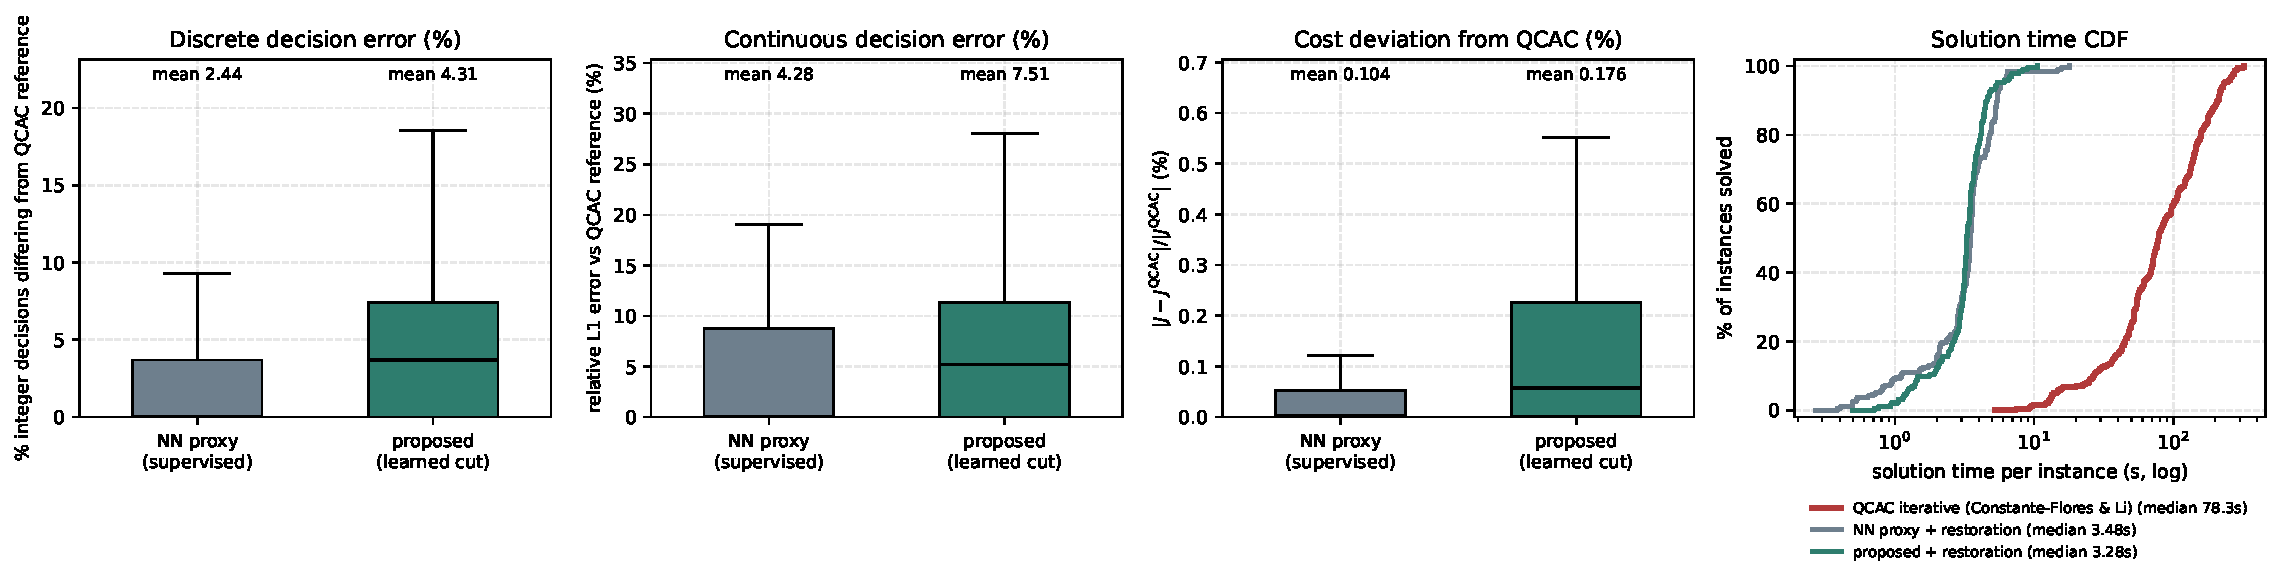
\includegraphics[width=\linewidth]{../figures/QUAD_case118.pdf}\\[2pt]
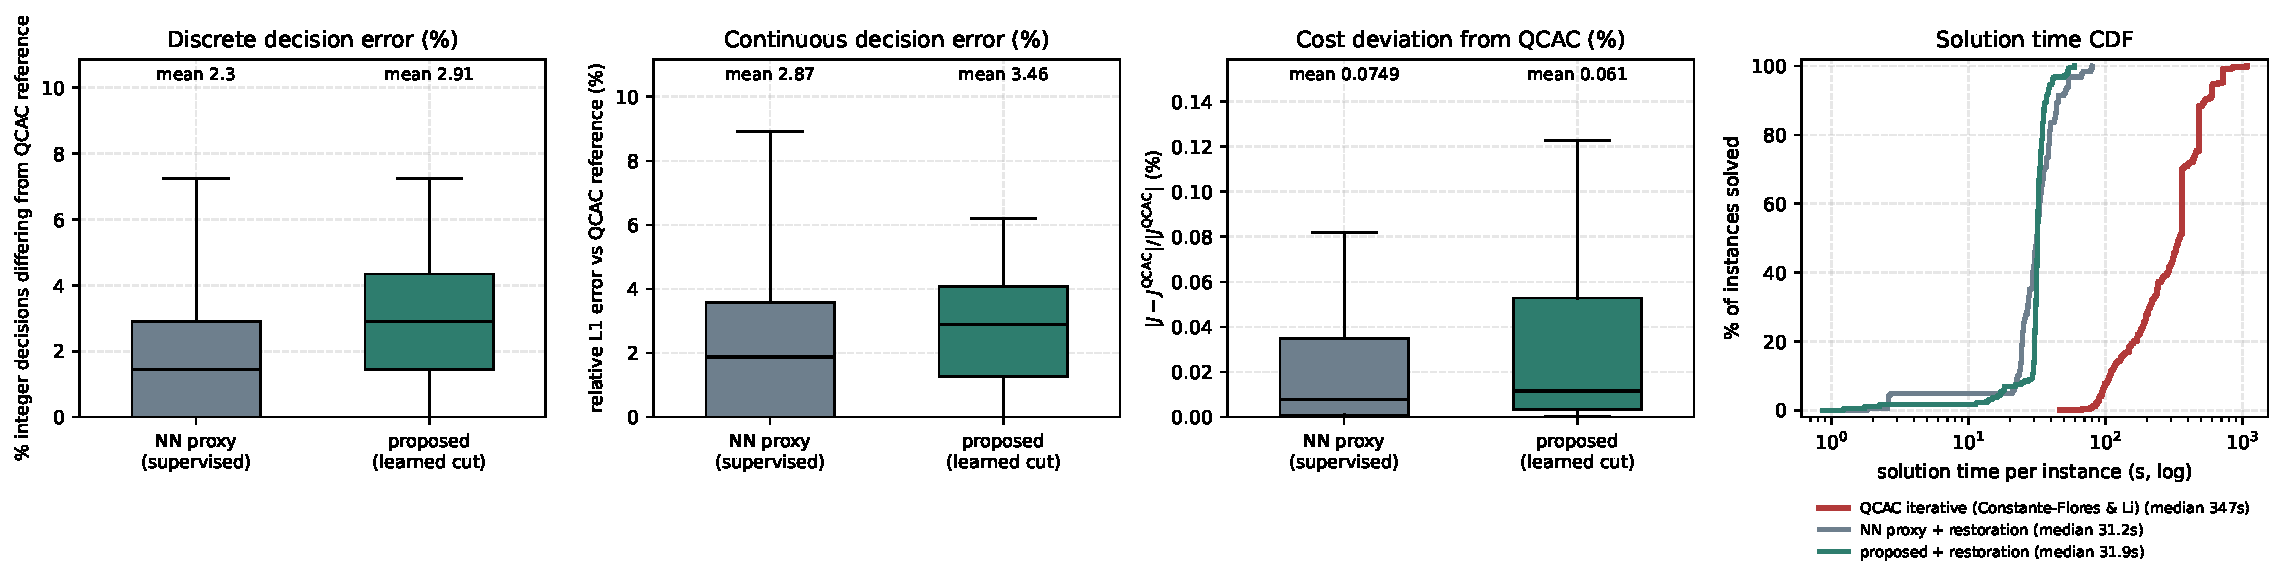
\includegraphics[width=\linewidth]{../figures/QUAD_case300.pdf}\\[2pt]
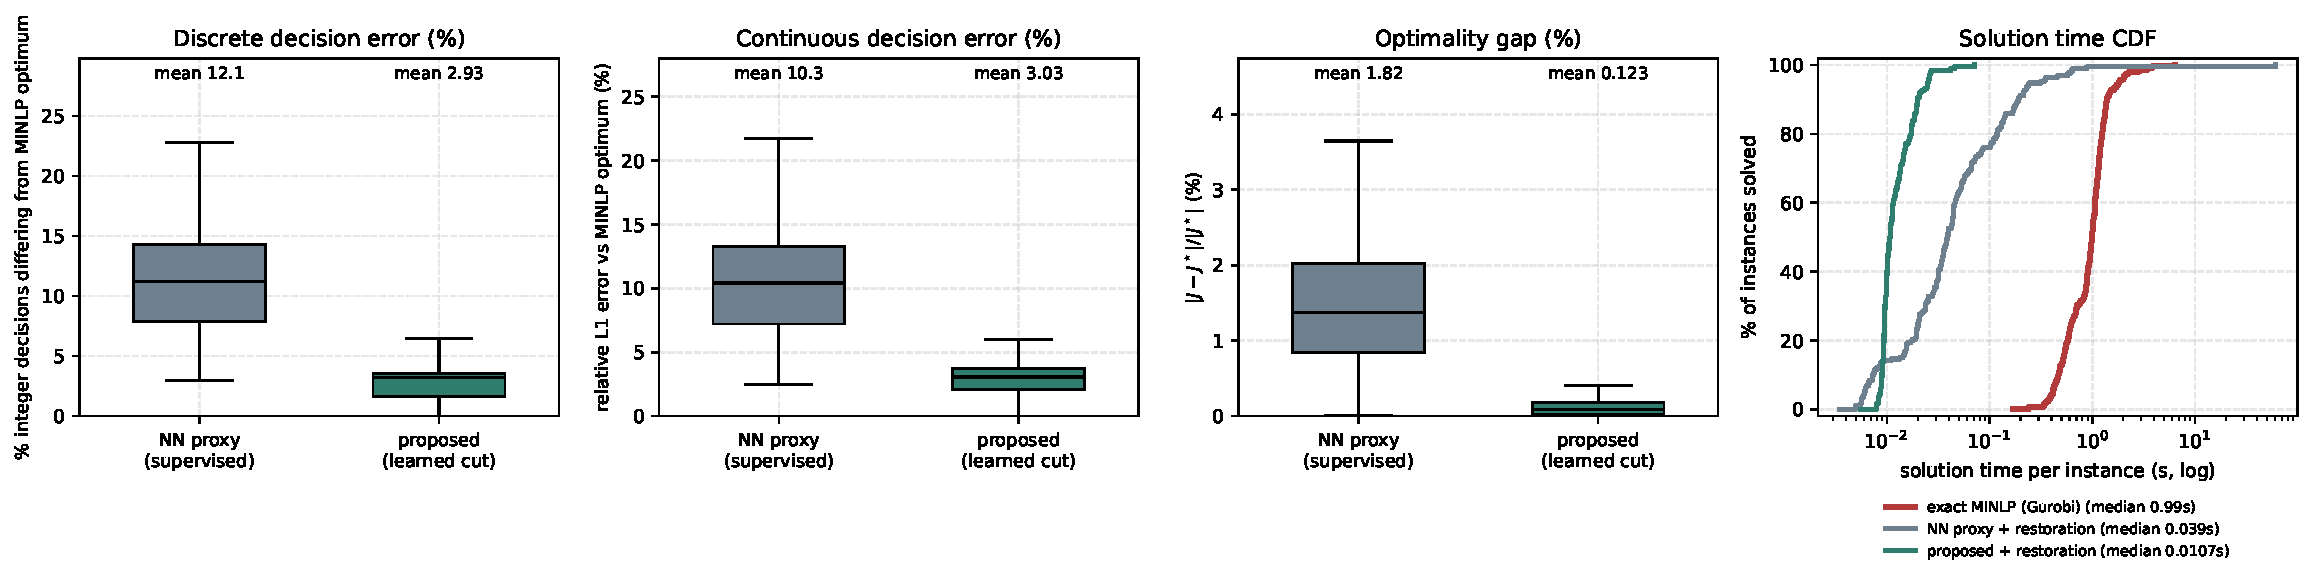
\includegraphics[width=\linewidth]{../figures/QUAD_hybrid_vehicle.pdf}
\caption{Held-out test results, top to bottom: case118, case300, hybrid vehicle. Box plots of discrete error, continuous error and absolute cost gap (whiskers at 1.5 IQR, outliers hidden) for the supervised NN proxy and the learned cut, and the CDF of per-instance solution time, including the reference solver.}
\label{fig:quad}
\end{figure}

\Cref{tab:main} and \cref{fig:quad} report the held-out results.

\paragraph{Speed.} On every case the learned surrogate solves one conic program per instance instead of a sequence of mixed-integer solves. Median time falls from \REFtimeA\,s to \OURtimeA\,s on case118 (\SPDA$\times$), from \REFtimeB\,s to \OURtimeB\,s on case300 (\SPDB$\times$), and from \REFtimeV\,s to \OURtimeV\,s on the vehicle problem (\SPDV$\times$). On unit commitment most of the remaining time is restoration (pricing candidate commitments), which the proxy pays equally; its median time is \PXtimeA\,s and \PXtimeB\,s.

\paragraph{Vehicle.} The learned cut is within \OURgapV\% of the global optimum on average, with \OURdiscV\% discrete and \OURcontV\% continuous error. The supervised proxy, given the optimal schedules and the same $\ell_1$ projection, has \PXgapV\% gap, \PXdiscV\% discrete and \PXcontV\% continuous error, so the learned cut is \VRATIO$\times$ more accurate in cost. We attribute the gap to the proxy having to regress 30 coupled integer modes from a 30-dimensional demand profile with 144 examples, whereas in our surrogate the energy dynamics are enforced exactly by the relaxation.

\paragraph{AC unit commitment.} On case118 the supervised proxy is more accurate than the learned cut on all three metrics: \PXgapA\% against \OURgapA\% mean cost deviation, \PXdiscA\% against \OURdiscA\% discrete and \PXcontA\% against \OURcontA\% continuous error. Both take about the same time (median \PXtimeA\,s against \OURtimeA\,s), since restoration dominates. Our mean is driven by a tail of instances; the median deviation is $0.058\%$. On case300 the learned cut has the lower mean cost deviation (\OURgapB\% against \PXgapB\%; signed $-0.029\%$, i.e.\ on average slightly \emph{cheaper} than the QCAC reference), while the proxy reproduces the reference decisions more closely (\PXdiscB\% against \OURdiscB\% discrete and \PXcontB\% against \OURcontB\% continuous error). Lower cost with a larger decision deviation is what the two objectives predict: the proxy imitates the reference decisions, while our loss contains only cost, and on these systems several commitments have nearly equal cost. The labels the proxy trains on cost \LABELHA\,h (case118) and \LABELHB\,h (case300) of reference-solver time; our method uses none of it.

\subsection{Gradient quality}
\label{sec:gradients}
\Cref{tab:grad} collects the gradient checks behind the method. Every check compares against central finite differences whose convergence is verified first (agreement between step sizes $10^{-3}$ and $3\times10^{-4}$). With an unconverged reference ($h=10^{-2}$), the correct layer read as 99\% wrong. On case118 the exact layer's gradient of a fixed loss with respect to the cut has cosine $0.9996$ with the reference from a single solve plus one sparse LU ($0.10$\,s). A Gaussian-perturbation estimator~\citep{berthet2020perturbed} at the settings used for training ($\sigma=0.15$, $P=2$ perturbation pairs, 4 solves) reaches $0.41\pm0.25$, and the best setting in a $4\times6$ sweep reaches $0.82$ with 64 solves. Larger $\sigma$ is worse at every sample size (bias), and accuracy grows only like $\sqrt P$ (variance). On case300 the gap is wider ($0.9995$ against $0.18$ and at best $0.52$). In training, learning the linearization point $V$ with the smoothed estimator made the loss rise on both systems while the exact gradient made it fall.

\begin{table}[t]
\centering\small
\caption{Gradient validation against converged finite differences (cosine, or relative error where noted).}
\label{tab:grad}
\begin{tabular}{@{}llc@{}}
\toprule
Quantity & Case & Agreement \\
\midrule
Exact layer, $\partial\ell/\partial b$ (1 solve) & case118 / case300 & $0.9996$ / $0.9995$ \\
Smoothed estimator, training setting (4 solves) & case118 / case300 & $0.41$ / $0.18$ \\
Smoothed estimator, best of sweep (64 solves) & case118 / case300 & $0.82$ / $0.52$ \\
Layer 1 (relaxation w.r.t.\ cut), held out & case118 / case300 & $0.944$ / $0.969$ \\
Layer 2 (priced cost w.r.t.\ commitment) & case118 & $0.990$ \\
Soft rounding with reserve threshold~\eqref{eq:rank1} & case118 & $1.000000$ \\
End-to-end $\partial\ell/\partial b$ through the chain & case118 / case300 & $0.962$ / $0.940$ \\
End-to-end $\partial\ell/\partial V$ & case118 & $0.864$ \\
Vehicle, $\partial\ell/\partial A$, $\partial\ell/\partial b$ (rel.\ error, 10 instances) & vehicle & median $0.02\%$ / $0.01\%$ \\
\texttt{cvxpylayers} on the QCAC relaxation & case118 & 97\% relative error \\
\bottomrule
\end{tabular}
\end{table}

\section{Discussion and limitations}
\label{sec:discussion}
\emph{Reference quality.} On AC unit commitment the reference is the QCAC iterative heuristic, an upper bound from an inner approximation. Deviations of either sign are deviations from that heuristic, not optimality gaps, and a discrete ``error'' can be a different commitment of equal or lower cost.
\emph{Labels versus no labels.} A supervised proxy and our method answer different questions. The proxy imitates a reference and needs that reference for every training instance. Our method optimizes deployed cost directly and needs only parameter samples, so it applies where reference solutions are unavailable or too expensive to generate. Where labels are cheap and the decision map is easy to regress, imitation can be the stronger choice; our case118 results show this.
\emph{Restoration.} Both methods rely on restoration to produce integer-feasible solutions, and its design (priority order, repair budget) materially affects the final numbers. Restoration is excluded from the training map, so training optimizes an upper bound on deployed cost.
\emph{Training signal on case300.} On case300 the label-free validation loss was lowest within the first five epochs for all four seeds, so the selected models are close to their initialization. The training objective (cost at a soft-rounded commitment) is not yet a faithful enough proxy for deployed cost on this system.
\emph{Scale.} Each training step solves two conic programs and two sparse KKT systems per instance on a CPU. Training takes about an hour per seed at case300 size, which is comparable to DFSM's reported training time but grows with problem size.

\section{Conclusion}
\label{sec:conclusion}
Learning parametric cutting planes is a natural way to turn a slow mixed-integer solve into a fast convex one while keeping the original constraints. We showed that these cuts can be learned by gradient descent through an exact differentiable conic layer, without any optimal solutions, for MINLPs with second-order-cone relaxations, including nonconvex AC unit commitment, where the network also learns where to convexify. The key practical obstacle was not the idea but the gradient: the relaxations are degenerate, off-the-shelf layers return wrong derivatives, and smoothed estimators are too noisy to train on. With a regularized direct KKT solve and depth-anchored cuts, the exact gradient is accurate and training is stable. The resulting surrogates solve \SPDA--\SPDV$\times$ faster than the reference solvers and, on the vehicle problem, are an order of magnitude more accurate than a supervised proxy trained on optimal solutions.

\bibliographystyle{plainnat}
\bibliography{refs}

\appendix
\section{Implementation details}
\label{app:impl}
\paragraph{Relaxation as an SOCP.} Handed to Gurobi, the continuous QCAC relaxation of case118 is treated as nonconvex: Gurobi does not certify the rotated-cone form of the rank-one strengthening and runs spatial branch-and-bound, hitting a 120\,s limit. The same model is an SOCP and Clarabel solves it in $0.06$--$0.10$\,s with an identical objective. This is what makes training feasible: each step solves two conic programs per instance. The SOC strengthening is necessary. Without it the slack still vanishes but the voltage products leave the rank-one manifold, and the relaxation returns a cost below the proven optimum on a test instance.
\paragraph{Layer 2 failures.} A soft commitment that only just meets the reserve can make the priced AC problem infeasible. During training we escalate the reserve margin (unit commitment) or lower the threshold (vehicle) and retry, the differentiable analogue of upward repair.
\paragraph{Regularization constants.} $\varepsilon=10^{-8}$ (layer 1) and $10^{-10}$ (layer 2) at $\rho=10^6$, each chosen on a validation split of instances. Sharing one value between the layers cut layer 2's gradient cosine from $0.9999$ to $0.42$, so the constant is per layer.
\paragraph{Code.} The released code (cone layer, both case studies, trained AC unit-commitment checkpoints, reference pools and all result files) reproduces every number in this paper.

\end{document}
